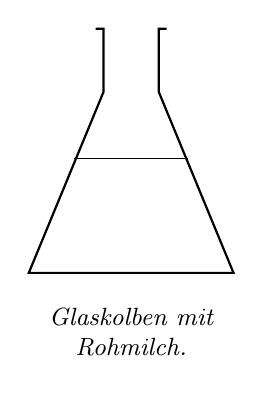
\begin{tikzpicture}[line width=0.8pt]
  % Erlenmeyer (Glaskolben) flask
  \draw
    (-0.35,3.0) -- (-0.35,3.1) -- (-0.45,3.1)
    (-0.35,3.0) -- (-0.35,2.3)
    -- (-1.3,0.0) -- (1.3,0.0)
    -- (0.35,2.3) -- (0.35,3.0)
    (0.35,3.0) -- (0.35,3.1) -- (0.45,3.1);
  % liquid (milk) surface line
  \draw[line width=0.4pt] (-0.72,1.45) -- (0.72,1.45);
  % caption
  \node[font=\itshape\small,align=center] at (0,-0.75)
    {Glaskolben mit\\ Rohmilch.};
\end{tikzpicture}
